\iffalse 
\svnInfo $Date: $
\svnInfo $Revision: $
\svnInfo $Author: $
\svnInfo $HeadURL: $
\svnInfo $Id: $
\fi

\RequirePackage{fix-cm,cmap,hyphsubst}
\HyphSubstLet{ngerman}{ngerman-x-latest}

\documentclass[%
  a4paper
  ,ngerman
  ,notumble
]{leaflet}

\usepackage[T1]{fontenc}
\usepackage{selinput}
                     
\SelectInputMappings{
adieresis={ä},
germandbls={ß},
Euro={€},
}

\usepackage{fixltx2e}
\usepackage{babel}
\usepackage[babel]{csquotes}

\usepackage{%
  ellipsis
  %,ragged2e,
  ,multicol
  ,nicefrac
  ,xspace
  ,icomma
  ,paralist
}

\makeatletter
\xspaceaddexceptions{\check@icr}
\makeatother

\usepackage{lmodern,upgreek,wasysym,eurosym}

\usepackage{microtype}

\usepackage[%
  pdfa,
  pdfencoding=auto,
  pdfusetitle,
 ,pdfpagemode=UseNone
 ,pdfstartview=FitH
]{hyperref}
\hypersetup{pdfprintscaling=None}

\renewcommand{\familydefault}{\sfdefault}

\def\hksqrt{\mathpalette\DHLhksqrt}
\def\DHLhksqrt#1#2{\setbox0=\hbox{$#1\sqrt{#2\,}$}\dimen0=\ht0
\advance\dimen0-0.2\ht0
\setbox2=\hbox{\vrule height\ht0 depth -\dimen0}%
{\box0\lower0.4pt\box2}}

\title{Neo}
\author{Ergonomisches Tastaturlayout}
\date{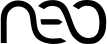
\includegraphics[height=3ex]{neo_logo}}

\usepackage{blindtext}





\begin{document}

\maketitle
\begin{itemize}%{compactitem}
\item ein Layout für Programmierer, Vielschreiber und Tippneulinge
\item ein Blick über den Tellerrand
\item eine Tastatur optimiert auf die die deutsche Sprache
\end{itemize}%{compactitem}

\vfill

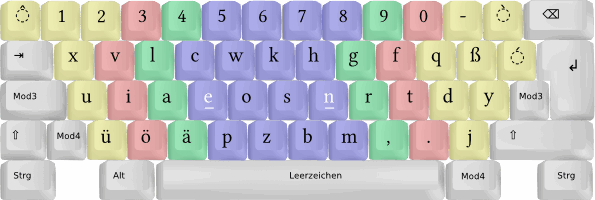
\includegraphics[width=\textwidth]{tastatur_neo_Ebene1}

\vfill

\begin{center}
\emph{In dubio pro Neo}.
\end{center}
\newpage
\section{Das Problem}

Die meisten von Euch benutzen eine sogenannte QWERTZ"=Tastatur (nach den ersten Buchstaben der oberen Reihe links) und sind der Meinung, diese Tastatur wäre gut so und hätte sich irgendwie nach ergonomischen Gesichtspunkten entwickelt. Falsch.

Das QWERT-Tastaturlayout wurde 1870 von Christopher Sholes konstruiert, um ein Verhaken der Typenhebel auf mechanischen, frühen Schreibmaschinen zu vermeiden und die Tippgeschwindigkeit zu hemmen. Schon Sholes selbst wusste, dass diese Anordnung auf modernen Tastaturen kontraproduktiv ist.

QWERTZ ist ein Relikt der Steinzeit. Während die Computerwelt rasant voranschreitet und die Menschen von Softwareergonomie reden, beharren sie weiterhin auf einen 140"=jährigen Fehler -- und das auch noch bei der wichtigsten Mensch"=Maschine"=Schnittstelle. Eigentlich sollte es doch indiskutabel sein, diesen Missstand zu beseitigen, egal wie lange es \enquote{funktioniert} hat.

\section{Die Lösung}
Neo ordnet die Buchstaben der Tastatur neu, die wichtigsten liegen auf der Grundreihe. Etwa die Vokale \texttt{uiae} auf der linken, die
häufigsten deutschen Konsonanten \texttt{nrtd} auf der rechten Hand.

Dabei könnt Ihr eure alte Tastatur behalten, geändert wird lediglich das Layout, also die Software. Der Aufwand des Umlernens des Layouts auf Neo hält sich dabei in Grenzen. Es kostet nur Überwindung.

\subsection{Vorteile von Neo}
\begin{compactitem}
\item schnellere Tippgeschwindigkeit durch bessere Position der häufigen Buchstaben
\item keine Überlastung der linken Hand wie bei QWERTZ
\item Programmier- und Sonderzeichen wie \texttt{/ \textbackslash\ [ ] \$ >~=} sind gut erreichbar
\item neue Zeichen wie \texttt{„ “ » « ?‘ \cent\ $\varsigma$ \female}
\dots\ können direkt eingegeben werden
\item genauso mathematische Zeichen wie $\Delta\,\partial\,\int\,\hksqrt{}\,\upalpha\,\upbeta$ -- auch in \LaTeX!
\item Ziffernblock, Steuerkreuz $\leftarrow\,\uparrow\,\rightarrow\,\downarrow$
und Befehlsfeld auch auf der Haupttastatur
\end{compactitem}

\section{Wie Neo funktioniert}
Um die umfangreichen Funktionalitäten bieten zu können, benötigt Neo zusätzliche \enquote{Ebenen}. QWERTZ verwendet fast nur zwei, die erste für die Klein- und die Shift"=Ebene für die Großbuchstaben. Dazu kommt noch AltGr für @, \textbackslash\ und \euro.

Neo erweitert diese Idee und bietet gleich sechs Ebenen. Die dafür nötigen Modifier (\enquote{Umschalttasten}) sind mit den kleinen Fingern gut erreichbar.

Wer will, braucht auch nur die ersten drei Ebenen zu nutzen und wird allein davon schon angenehm überrascht sein. Für \LaTeX\ etwa kann man nun den viel zu oft benötigten Backslash bequem per QWERTZ"=Raute~+ QWERTZ-A erreichen. Und wer meint, dass das US"=Layout dies genauso gut
schafft, hat wohl noch nie deutsche Umlaute getippt ;-)

Die vierte Ebene ersetzt euch alles jenseits des Tastaturhauptfeldes, wie etwa den Zahlenblock, den z.\,B. Notebooks nicht haben. Und last but not least: Die griechischen Kleinbuchstaben und mathematischen Zeichen der 5.\,bzw.\ 6.\,Ebene, für deren Aktivierung Ihr zwei Modifier gleichzeitig drücken müsst, sind ein ungemein wertvolles Feature für die, die es nutzen.

\vfill

\hspace*{2ex}
\includegraphics*[width=2.1\linewidth]{neo-druckvorlage}

\section{Was nun zu tun ist}
Installationsanleitungen für alle gängigen Plattformen, Hilfestellungen und FAQ findet Ihr auf der Neo-Seite und vor allem im hauseigenen Wiki: \url{wiki.neo-layout.org} 

Dort gibt es auch Verweise zu anderen alternativen Layouts, wie etwa das schon seit 1932 bestehende Dvorak oder das erst 2005 entwickelte RISTOME. 

Wenn Du willst, beschäftige Dich damit und triff Deine Entscheidung. Sollte sie pro Neo sein, empfehlen wir, dies auch konsequent durchzuziehen. Im Wiki findest Du zahlreiche Erfahrungsberichte und weitere Tipps.

Aber Vorsicht: Wer einmal Neo benutzt, wird nie wieder etwas anderes wollen.

\vspace{12.5em}
\emph{Der technische Fortschritt hat bereits gesiegt. Schließt Du Dich ihm heute an – oder erst, wenn schon alle anderen mitmachen?}

\newpage

\blindtext[6]
\end{document}
